\documentclass{amsart}
\usepackage[margin=3cm]{geometry}                % See geometry.pdf to learn the layout options. There are lots.
\geometry{letterpaper}                   % ... or a4paper or a5paper or ...
%\geometry{landscape}                % Activate for for rotated page geometry
\usepackage[parfill]{parskip}    % Activate to begin paragraphs with an empty line rather than an indent
\usepackage{float}
\usepackage{graphicx}
\usepackage{amssymb}
\usepackage{epstopdf}
\usepackage{siunitx}
\usepackage{subcaption}
\usepackage{setspace}
\usepackage{ wasysym }

\DeclareGraphicsRule{.tif}{png}{.png}{`convert #1 `dirname #1`/`basename #1 .tif`.png}
\graphicspath{{./img/}}

\title{Electron Spin Resonance}
\author{Caspar \textsc{Lant}} % Author name

\date{\today} % Date for the report

\begin{document}

\bigskip

\maketitle % Insert the title, author and date
\begin{center}

Intermediate Experimental Physics II\\
\vspace{1.5cm}

\begin{tabular}{l r}

Section: & 001\\
\\
Date Performed: & March $e^{i\phi}$, 2016 \\ % Date the experiment was performed
Date Due: & March $ \frac{d}{dx}\delta(x)$ , 2016\\
\\
Partner: & Neil Saddler\\ % Partner names
Professor: & Prof. Andrew Kent\\
Instructor: & David Mykytyn % Instructor/supervisor
\end{tabular}
\vfill
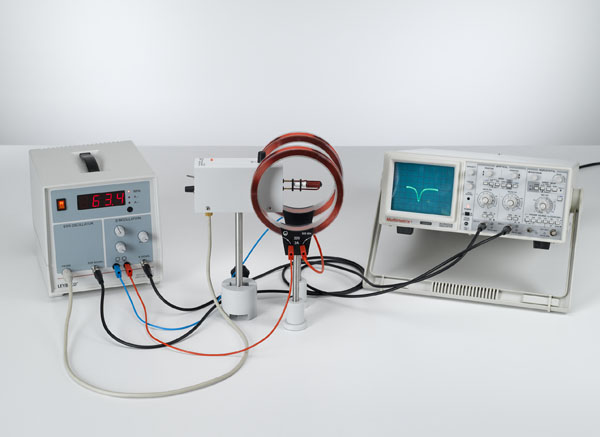
\includegraphics[width=.7\textwidth]{diagram.jpg}
\end{center}
\vfill
\pagebreak
\setstretch{1.5}
\paragraph{\textbf{The Objective} of today's experiment was to measure $\delta B$ as well as the famous g-factor, a quantity that relates the resonant frequency of an electron's spin moment to the strength of an external magnetic field.}

\section{Theoretical Background/ Abstract}
Electron Spin Resonance is a effect that occurs when materials containing unpaired electrons find themselves in the presence of an external magnetic field. Electron spin resonance is similar to the nuclear spin resonance (the subject of another experiment in this course), but instead of relating to the excited spins of atomic nuclei, this type of resonance describes the spin states of excited electrons. Depending on who you ask (and specifically their political allegiances), electron spin resonance was discovered by either a Soviet physicist by the name of Yevgeny Zavoisky, or by the Allied physicist Brebis Bleaney.

Electrons are partially defined by their magnetic moment and spin number, both of which are quantized. The spin number of all electrons, and fermions in general is 1/2. The magnetic moment of an electron is defined by the following:
\begin{equation}
    {\bf \mu}_S = \dfrac{g_S \mu_B S}{\hbar}
\end{equation}
Where $S$ is the electron's spin (1/2) and $g_s$ is its g-factor, which is a quantity we hope to arrive at later in this lab (but for now we'll set it equal to 2) $\mu_s$ is the Bohr magneton, equal to approximately $9 \times 10^{24}$ Joules per Tesla.
% As you can see, the magnetic moment of an electron points in the same ``direction" as its spin.
The energy of an electron in the presence of and external magnetic field $B_0$ depends on the alignment of its spin magnetic moment relative to the direction of $B_0$. Uncoupled electrons in a material such as DPPH (2,2-diphenyl-1-picrylhydrazyl, shown in figure \ref{fig:DPPH}) have little trouble setting their magnetic moments either parallel or antiparallel to the magnetic field. The energy of such an electron is given by equation \ref{eq:energy}.
\begin{equation}
    E = m_sg\mu_BB_0
    \label{eq:energy}
\end{equation}
$m_s$ differs by a sign depending on it's alignment relative to $B_0$, making the difference in energy between the parallel and the antiparallel state. This difference is defined in equation \ref{eq:energy_diff} and depicted in figure \ref{fig:energy_diff}.
\begin{equation}
    \Delta E = h\nu = g\mu_B B_0
    \label{eq:energy_diff}
\end{equation}
\begin{figure}
    \centering
    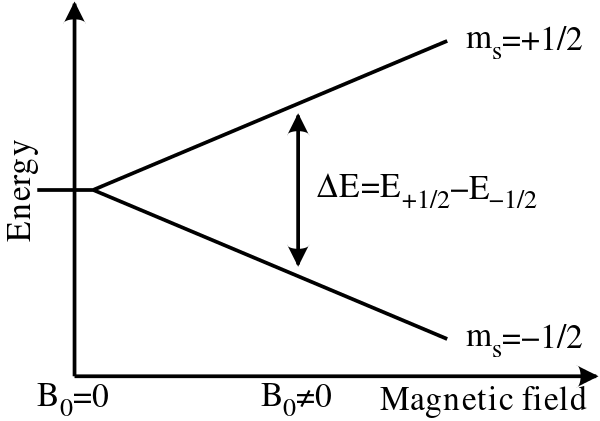
\includegraphics[width=0.4\textwidth]{splitting.png}
    \caption{Energy Splitting}
    \label{fig:energy_diff}
\end{figure}
Where $\nu$ is the minimum frequency required to induce a state transition. This quantity, $\Delta E$ is referred to as the ``line width", and is related to factors such as the dipole-dipole interactions between uncoupled electrons' magnetic moments, as well as the interactions between a single electron and the internal magnetic fields intrinsic to the material. Other factors that can influence the energy line width are exchange interactions and spin-orbit coupling between two unpaired electrons. In DPPH, the material we will examine in this lab, it is electron exchange that most influences $\delta E$, and is another quantity that we will measure and discuss.

The reorientation of the spin of a particle in the presence of an external magnetic field is an transition termed spin flip. The following equation relates the outer product of $\mu$ and $B$, which is typically minimized such that the two vectors point in the same direction, to the cross-product of the ``angular momentum"  of an electron (in quotations because electrons are point particles) and the Larmor angular frequency, $\omega_L$, which describes the electron's precession.
\begin{equation}
    \vec \mu \times \vec B = \omega_L \times \vec L
\end{equation}
It turns out that the angular frequency $\omega_L$ is precisely the frequency that initiates a spin flip, and holds the same value as $\nu$ in equation \ref{eq:energy_diff}! This is very exciting. It is the relationship between this quantity and the applied magnetic field that we are interested in learning about in this lab. We will find that the two are directly proportional, and differ by a constant $g$. The same $g$, in fact, that we have seen in equation \ref{eq:energy}!

In order to measure produce our external magnetic field, we will use a device known as a Helmholtz coil. A Helmholtz coil is, in effect, two coaxial coils (solenoids) of equal radius separated by their radius. In allowing an equal magnitude of current to flow through each coil, a fairly uniform magnetic field can be produced, as seen in figure \ref{fig:coils}. By placing our sample directly between the two coils, we can be fairly confident in our measure of magnetic field strength, which is given by equation \ref{eq:field}.

\begin{figure}
    \begin{minipage}{0.45\textwidth}
        \centering
        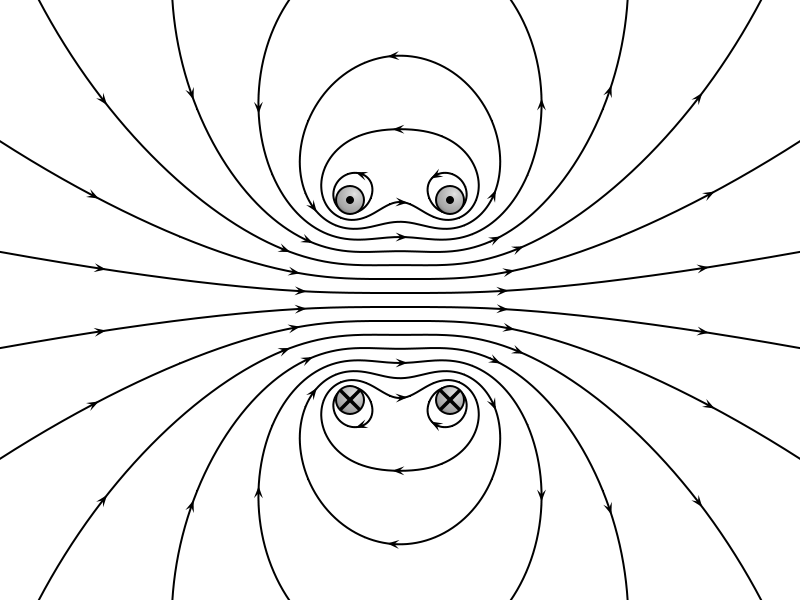
\includegraphics[height=5cm]{coils.png}
        \caption{Field Lines}
        \label{fig:coils}
    \end{minipage}
    %
    \begin{minipage}{0.45\textwidth}
        \centering
        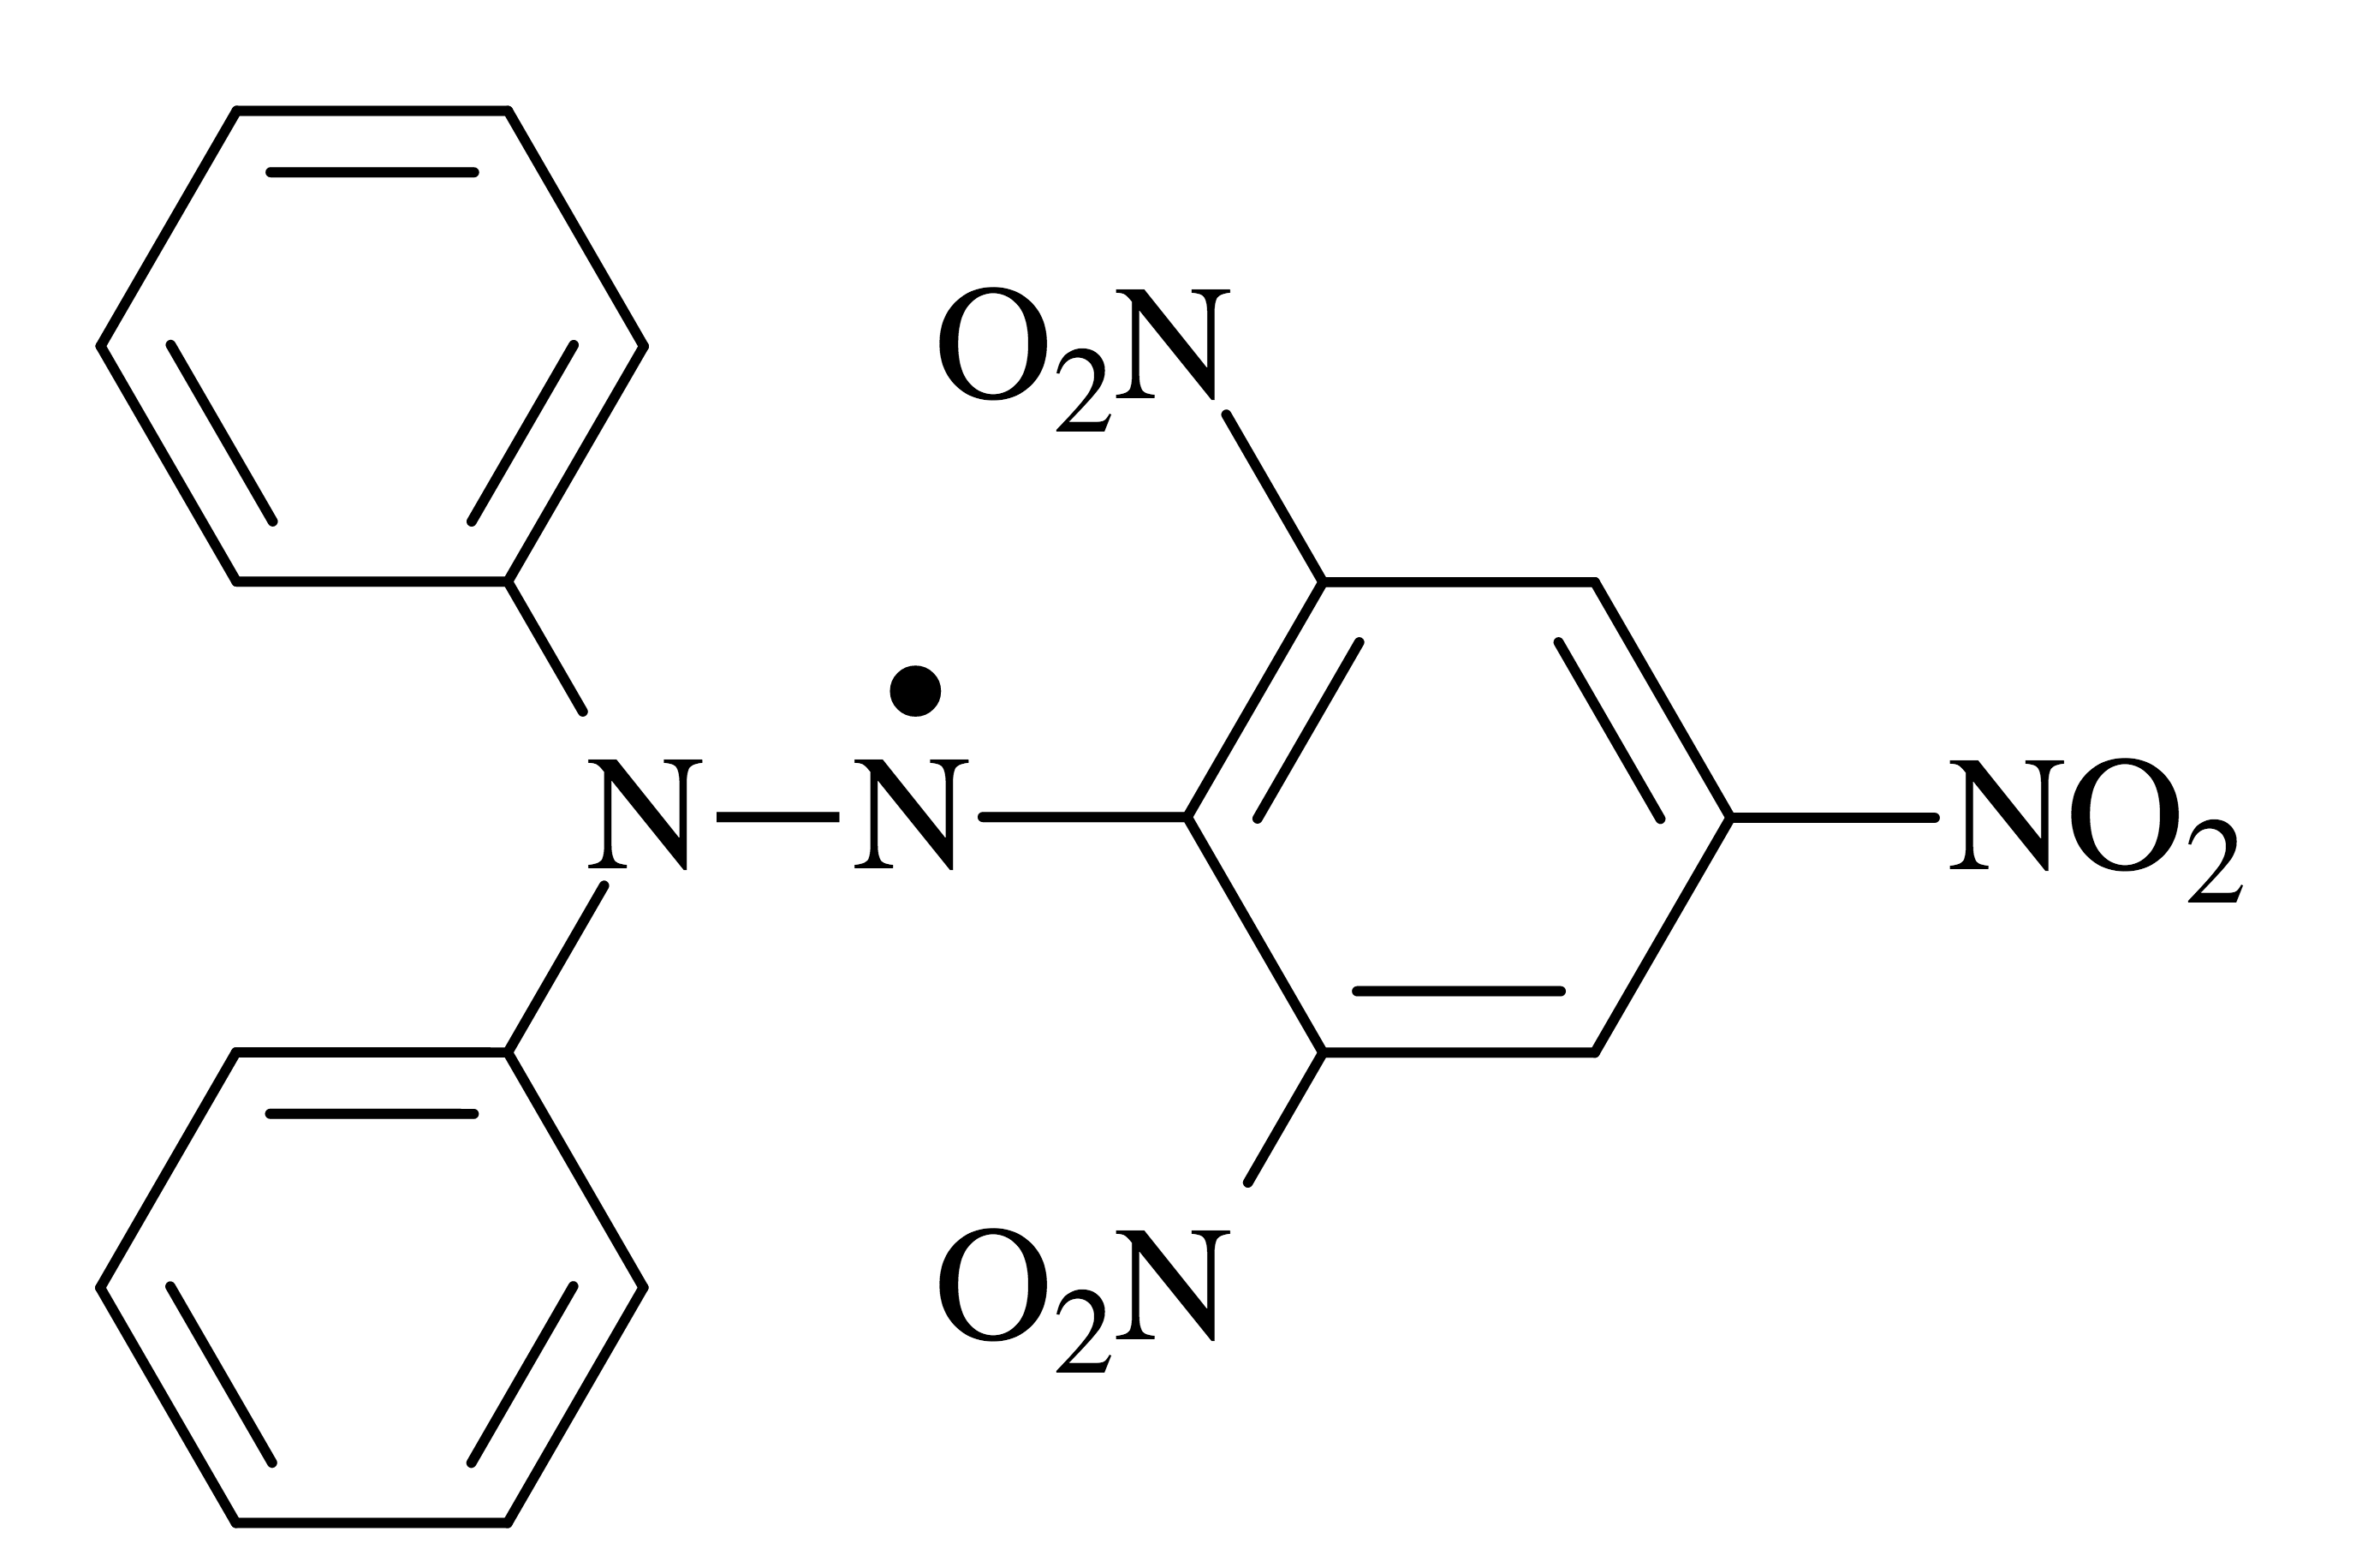
\includegraphics[height=5cm]{dpph.png}
        \caption{DPPH}
        \label{fig:resonance}
    \end{minipage}
\end{figure}

\begin{equation}
    \dfrac{\mu_0 N}{2R}\left(\dfrac{4}{5}\right)^{\frac{3}{2}}(2I_0) = 2.115(2I_0)mT
    \label{eq:field}
\end{equation}

\section{Experimental Procedure}
\begin{enumerate}
    \item Plug everything in in the manner depicted in the illustration on the cover page and ensure that all measurement devices are powered off.
    \item Carefully plug the largest RF coil into the RF unit.
    \item space the solenoids by a distance of 6.8cm.
    \item Place the sample into the coil and place it in the center of the volume formed by each solenoid.
    \item Make sure that $U_0$ is set to zero, and $U_{\rm mod}$ is set to the second scale marking.
    \item Turn on all devices. The oscilloscope should be set for two channel operation with channel one triggering.
    \item Set the frequency adjuster on the RF unit to 15 MHz. The Amplitude should be at its maximum.
    \item Now, increase the DC coil voltage $U_0$ until resonances are seen on the oscilloscope's phosphor screen. This will take the form of a nice, symmetric ``v"-curve, similar to the Gaussian function $-e^{-x^2/a}$ lol.
    \item Increase the frequency of the RF transmitter in increments of 15 MHz until the RF coil saturates. When you've reached the maximum frequency of the RF coil in the transmitter, turn off the transmitter and swap it out with a smaller one.
    \item You're done!
\end{enumerate}

\section{Graphs and Tables}

\begin{table}[H]
    \centering
    \caption{Voltage vs. Deflection}
    \label{table:deflection}
    \begin{tabular}{c|c|c|c}
        $f$ (MHz)&$I_0$ (A) &$2I_0$ (A) &$B$(mT) \\ \hline
        30.7     & 0.644    & 1.288     & 2.724  \\
        35.0     & 0.731    & 1.462     & 3.092  \\
        40.0     & 0.880    & 1.760     & 3.722  \\
        45.0     & 0.993    & 1.986     & 4.200  \\
        50.0     & 1.112    & 2.224     & 4.704  \\
        55.0     & 1.205    & 2.410     & 5.097  \\
        60.0     & 1.317    & 2.634     & 5.571  \\
        65.0     & 1.442    & 2.884     & 6.100  \\
        70.0     & 1.534    & 3.068     & 6.489  \\
        75.0     & 1.595    & 3.190     & 6.747  \\
        80.0     & 1.692    & 3.384     & 7.157  \\
        85.0     & 1.765    & 3.530     & 7.466  \\
        90.0     & 1.917    & 3.834     & 8.109  \\
        95.0     & 2.035    & 4.070     & 8.608  \\
        100.0    & 2.067    & 4.134     & 8.743  \\
        105.0    & 2.221    & 4.442     & 9.395  \\
        110.0    & 2.293    & 4.586     & 9.699  \\
        100.0    & 2.412    & 4.824     & 10.203
    \end{tabular}
\end{table}

\begin{figure}[h]
    \centering
    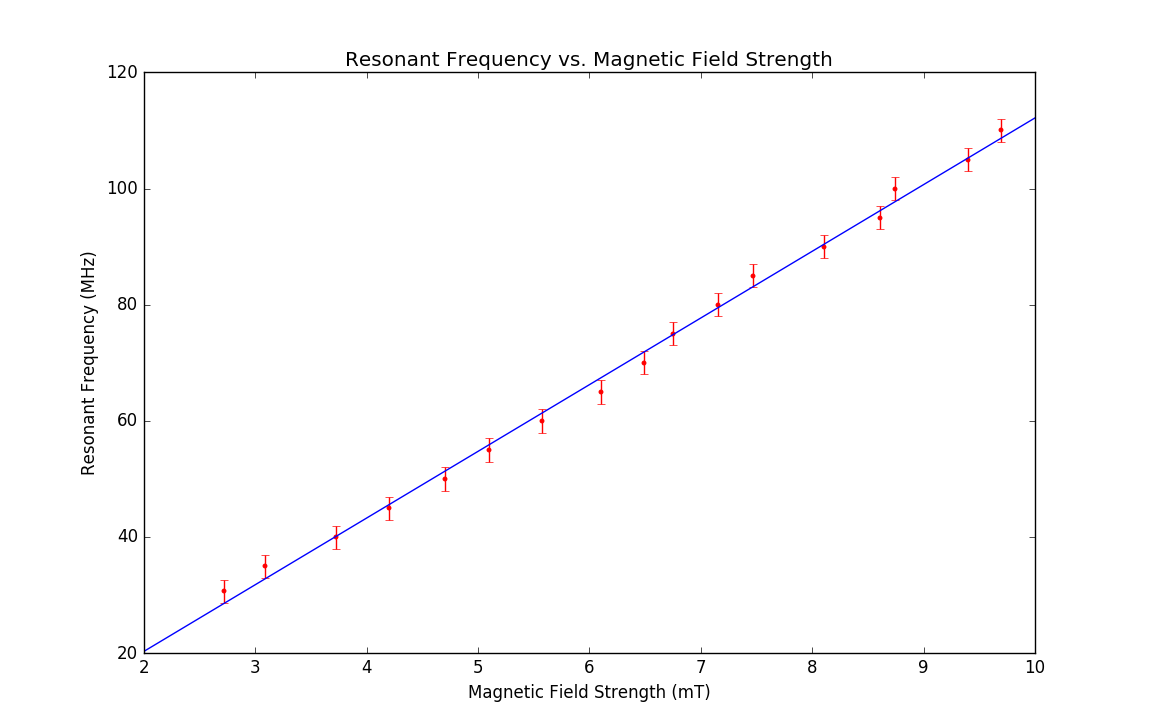
\includegraphics[width=\textwidth]{fitted.png}
    \caption{Finding $g_s$}
\end{figure}

I left our last measurement out of the fit, because it was a clear out-lier. Accounting for our error bars on resonant frequency (given by the number of significant figures in the display of frequency on the RF transmitter), our each data point fits snugly on my best-fit line.

\section{Analysis}
The slope of our fit line is 11.5, while its y-intercept is -2.6. The slope is equal to $\frac{\nu}{B}$, our frequency divided by the magnetic field strength. It has units MHz/mT. We can rearrange equation \ref{eq:energy_diff} to find $g$:
\begin{equation}
    g = \frac{h\nu}{\mu_B B}
\end{equation}
as stated previously, the Bohr magneton has a known value of $9.27400968\times10^{−24}$, making $g$ 0.82, which is upsettingly small. Our uncertainty in $g$ is given by the following expression from Taylor:
\begin{equation}
    \delta g = \delta{\rm slope} = \sqrt{\left(\frac{\delta\nu}{\nu}\right)^2 + \left(\frac{\delta B}{B}\right)^2}
\end{equation}
Which gives us an uncertainty of $\pm 0.35 {\rm MHz/mT}$, or not enough to put us within the expected value of $g \ \frownie$. Such a large error must be accounted for, but I am having trouble thinking of a source that would give us such a wild degree of uncertainty. As I said before, there is very low variance in $\frac{\nu}{B}$, which leaves even less room for uncertainty in $g$. I've combed over my calculations and have failed to find any mis-steps. This is very strange. The uncertainty in magnetic field strength, $\delta B$, is given by the following:
\begin{equation}
    \delta B = |B|\sqrt{\left(\frac{\delta a}{a}\right)^2 + \left(\frac{\delta I_0}{I_0}\right)^2}
\end{equation}
Which gives us an uncertainty of $\pm 0.49 {\rm mT}$, making $\delta B$ itself equal to $1.08\pm0.49 {\rm mT}$. 

\section{Questions}
\begin{enumerate}
    \item {\textit{The manufacturer designed this experiment with the coils connected in parallel. A series connection would be better. Why?}
    \begin{quote}
        A series connection would ensure that both coils received the same current, producing a more-uniform magnetic field.
    \end{quote}}
    \item {\textit{The p-p modulation current $\delta(2I_0)$ for the half-width $\delta$B is obtained from Where does the divisor 10 come from?}
    \begin{quote}
        The oscilloscope is set to 0.1 Volts per division.
    \end{quote}}
    \item {\textit{In the method given for measuring $\delta$B, the scope controls are not used in a calibrated mode. Why is this OK?}
    \begin{quote}
        We use a qualitative approach (namely, tuning the frequency until we see a ``nice-looking" resonance), to measure $\delta B$. Additionally, the measured values are relative to one another, so the oscilloscope setting are irrelevant provided that we do not change them during our measurement.
    \end{quote}}
    \item {\textit{Why is the multimeter set for DC amperes for measuring g and for AC amperes for measuring the line width?}
    \begin{quote}
        The line width is given by $I_{\rm rms}$, which is intrinsically a measure of alternating current. The value $g$ is dependent on $I_0$, which can only be determined with a direct current.
    \end{quote}}
    \item {\textit{Is there an RF electric field associated with the RF coil? If so, make a sketch of what the fields look like.}
    \begin{quote}
        There is no electric field associated with the RF coil, assuming it's been aligned properly and it is not malformed. I don't want to draw a diagram.
    \end{quote}}
\end{enumerate}



slope = 11.4794866225

\end{document}
